\documentclass[12pt,a4paper]{article}
\usepackage[a4paper,top=25mm,bottom=25mm,inner=18mm,outer=18mm,twoside]{geometry}
\usepackage[utf8]{inputenc}
\usepackage{amsmath}
\usepackage{amsfonts}
\usepackage{amssymb}
\usepackage{graphicx}
\usepackage{polski}
\usepackage{mathtools}
\usepackage[T1]{fontenc}
\usepackage{pdflscape}
\usepackage{graphicx}
\usepackage{caption}
\usepackage{subcaption}
\usepackage{floatrow}
\usepackage{float}
\usepackage{hyperref}
\usepackage{listings}
\usepackage{verbatim}
\usepackage{afterpage}
\DeclarePairedDelimiter{\ceil}{\lceil}{\rceil}

\newcommand{\ImgPath}{./img/}
\newcommand{\ResPath}{../badania/}

\lstset{
 basicstyle=\ttfamily\footnotesize
}

%\Figure{filename}{caption}{label}.
%\Figure{sciezka-do-pliku.png}{Opis opis}{labelka}
\newcommand\Figure[4][width=\linewidth]{%
  \begin{figure} [h!]
    \centering
    \includegraphics[#1]{\ImgPath /#2}
    \caption{#3}\label{#4}
  \end{figure}
}

\title{Rozmieszczanie kamer bezpieczeństwa}
\author{Wiktor Franus \\ Grzegorz Staniszewski}

\begin{document}
\maketitle
\tableofcontents

\newpage
\section{Treść zadania}
Jak optymalnie rozmieścić kamery monitoringu w ustalonym pomieszczeniu (rzut z góry), aby minimalną liczbą kamer móc obserwować dowolne miejsce (z uwzględnieniem maksymalnej dopuszczalnej odległości od kamery). W rozwiązaniu należy uwzględnić możliwość zapewnienia parametryzowanej redundancji - tzn. wymagania, aby każde miejsce było obserwowane przez co najmniej $n$ kamer.

\section{Założenia}
\begin{enumerate}

\item Pomieszczenie jest wielokątem zawierającym tylko kąty o mierze 90 lub 270 stopni. 
Pomieszczenie reprezentowane jest przez zbiór punktów (z I ćwiartki układu współrzędnych) podanych w formie listy. 
Połączenie tych punktów linią, zgodnie z ich kolejnością na liście, skutkuje otrzymaniem linii łamanej ograniczającej pomieszczenie.
Punkty podawane są w kolejności zgodnej z ruchem wskazówek zegara.
Pierwszy i ostatni punkt jest taki sami (należy domknąć pomieszczenie).
\item Kamery mają jednakowy zasięg reprezentowany przez kwadrat o parametryzowanej długości boku. 
Współrzędne kamery są jednocześnie współrzędnymi środka tego kwadratu. 
Kamera musi znajdować się wewnątrz pomieszczenia i nie przenika przez ściany.
\item Wnętrze pomieszczenia zdyskretyzowane jest do zbioru punktów o współrzędnych całkowitych poprzez nałożenie siatki o parametryzowanej gęstości.
\item Punkty leżące na krawędziach wielokąta opisującego pomieszczenie nie należą do jego wnętrza.
\end{enumerate}

\section{Przestrzeń przeszukiwań}
\begin{itemize}
	\item Elementem przestrzeni przeszukiwań jest wektor par liczb całkowitych oznaczających współrzędne kamer:\\
	$$[(x_1, y_1), ..., (x_i, y_i), ..., (x_k, y_k)]$$
	gdzie:\\
	$x_i$ - współrzędna x i-tej kamery,\\
	$y_i$ - współrzędna y i-tej kamery,\\
	$k$ - liczba kamer.
	\item Przejście do sąsiedniego elementu możliwe jest poprzez:
	\begin{itemize}
		\item zmianę położenia jednej z kamer na 2 sposoby (sposób
		ustalany jest na początku zadania):
		\begin{itemize}
		\item zmiana współrzędnych x lub y jednej z kamer o 1 jednostkę,
		\item przeniesienie jednej z kamer do innego punktu z wnętrza pomieszczenia
		wylosowanego zgodnie z rozkładem jednostajnym,
		\end{itemize}
		\item dodanie nowej kamery w losowym miejscu (rozkład jednostajny),
		\item usunięcie jednej kamery.
	\end{itemize}
	\item Przestrzeń ma strukturę grafową, w której każda krawędź odpowiada
	jednemu z wymienionych wyżej przejść między elementami przestrzeni.
\end{itemize}

\section{Funkcja celu}
Informacje znane dla danej instancji problemu: \\
$X$ - zbiór punktów reprezentujących wnętrze pomieszczenia. \\
$n_{kmin}$ - minimalna teoretyczna liczba kamer wymagana do pokrycia danego pomieszczenia
(obliczana jako stosunek liczności zbioru $X$ do liczby punktów pokrywanych przez 1 kamerę, zaokrąglany do jedności w górę),\\
%
\newline
Parametry funkcji celu: \\
$\alpha$ - zysk z pokrywania powierzchni pomieszczenia,\\
$\beta$ - koszt użycia nadmiarowej kamery, \\
$r_{min}$ - minimalna liczba kamer pokrywająca każde miejsce w pomieszczeniu. \\
%
\newline
Zadanie polega na maksymalizacji funkcji: \\
$$f(p, k, r) = \alpha * p - \beta * k - \frac{1}{r_{min}} * r $$ 
gdzie: \\
$p$ - stosunek liczby punktów pokrytych przez kamery do liczności zbioru $X$\\
$k$ - stosunek nadwyżki liczby kamer do $n_{kmin}$, obliczany wg. wzoru: \\
\indent $k = \frac{max(0, n_k - n_{kmin})}{n_{kmin}}$, gdzie $n_k$ - liczba kamer w aktualnym stanie \\\\
Parametr $r$ może być obliczany na dwa sposoby (sposób ustalany jest na
początku zadania):
\begin{itemize}
\item jako średni stopień niespełnienia warunku redundancji dla punktu z wnętrza pomieszczenia, obliczany wg. wzoru: \\
\indent $r = \frac{\sum_{x \in X}^{} max(0, r_{min} - r_x)}{|X|}$, gdzie $r_x
$ - liczba kamer pokrywających punkt $x$
\item jako maksymalne niespełnienie warunku redundancji spośród wszystkich
punktów z wnętrza pomieszczenia, wg. wzoru:\\
$r = max(0, r_{min} - r_x)$, gdzie $r_x$ - liczba kamer pokrywających punkt $x$, który jest najsłabiej pokrytym punktem.
\end{itemize}

%
\section{Przykład}
\begin{center}
	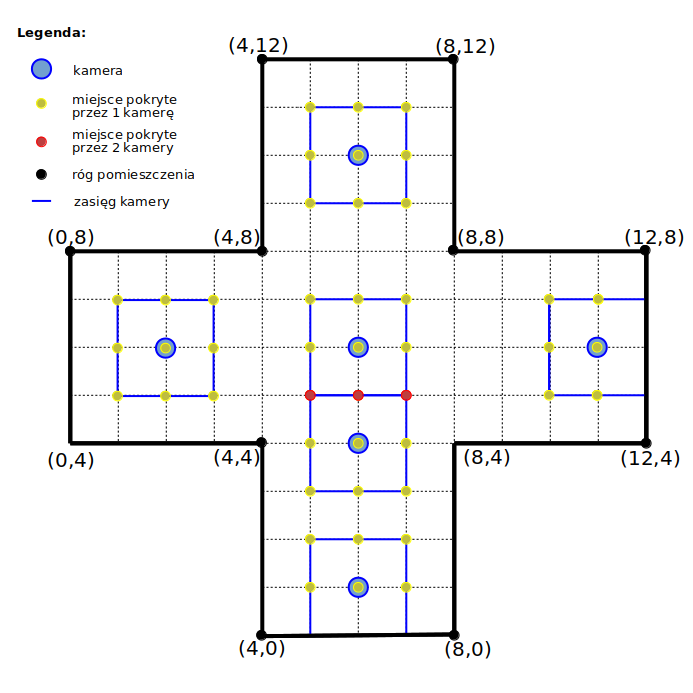
\includegraphics[scale=0.5]{img/example_2.png}
\end{center}


\begin{itemize}
	\item Wartości parametrów:\\
	$\alpha = 1$\\
	$\beta = 1$\\
	$r_{min} = 1$
	\item Informacje obliczone dla powyższego pomieszczenia:\\
	Rozmiar boku kwadratu reprezentującego zasięg kamery: 2\\
	Liczba punktów pokrywanych przez jedną kamerę: 9\\
	$|X| = 57$\\
	$n_{kmin} = \ceil{\frac{57}{9}} = 7$\\

	\item Obliczenie wartości funkcji celu dla stanu z rysunku:\\
	Liczba kamer użytych: 6\\
	Liczba punktów pokrytych przez kamery: 45\\
	$p = \frac{45}{57} = 0.7895$\\
	$k = \frac{max(0, 6-7)}{7} = \frac{0}{20} = 0$\\
	Parametr $r$ obliczany pierwszym sposobem:\\
	$r = \frac{45*0 + 12*1}{57} = \frac{12}{57} = 0.2105$\\
	$f(p, k, r) = 1*0.7895 - 1*0 - 1*0.2105 = 0.5790$\\\\
	Parametr $r$ obliczany drugim sposobem:\\
	$r = max(0, 1-0) = 1$\\
	$f(p, k, r) = 1*0.7895 - 1*0 - 1*1 = -0.2105$
\end{itemize}

\section{Metaheurystyka}
Element początkowy przestrzeni przeszukiwań jest zbiorem zawierającym $n_{kmin}$ kamer rozmieszczonych losowo wewnątrz pomieszczenia.\\
Do rozwiązania problemu użyjemy algorytmu symulowanego wyżarzania. Przy odpowiednio dobranych parametrach metoda ta, w porównaniu do algorytmów wspinaczkowych, daje większą szansę na znalezienie optymalnego rozwiązania, ponieważ zmniejsza ryzyko zatrzymania się w ekstremach lokalnych. W początkowej fazie przeszukiwania przestrzeni dopuszczalne jest przechodzenie do stanów gorszych (o mniejszej wartości funkcji celu). Wraz z rosnącą liczbą iteracji obszar poszukiwań jest ograniczany, a algorytm bardziej skupia się na poprawie bieżącego rozwiązania.

\section{Przewidywane wyniki pracy}
Przeprowadzona zostanie seria eksperymentów z różnymi wartościami parametrów $\alpha$, $\beta$, $r_{min}$ na kilku instancjach problemu (różne pomieszczenia). Dla ustalonych parametrów funkcji celu, sterować będziemy parametrami metaheurystyki, tj. funkcją wygaszania temperatury i jej
wartością początkową. Ponadto sprawdzimy dwa podejścia do zmiany położenia kamery oraz dwa sposoby obliczania parametru $r$ funkcji celu. Dla wybranej
instancji zadania sprawdzimy też wpływ gęstości siatki punktów z wnętrza
pomieszczenia na zachowanie metaheurystyki. Sporządzone zostaną wykresy przedstawiające wartość funkcji celu oraz liczbę użytych kamer w zależności od liczby wykonanych iteracji. 

\section{Implementacja}
Do realizacji zadania wykorzystaliśmy gotową implementację metaheurystyki zawartą w pakiecie simanneal w wersji 0.4.1,
której dokumentacja jest dostępna pod adresem \url{https://github.com/perrygeo/simanneal}.
Biblioteka implementuje algorytm symulowanego wyżarzania z wykładniczą funkcją wygaszania temperatury minimalizujący zadaną
funkcję celu. Z racji, że naszym zadaniem miało być maksymalizowanie opisanej w specyfikacji funkcji celu, musieliśmy zmodyfikować tę
funkcję, zmieniając jej znak na przeciwny. Poprawiony wzór na funkcję celu ma postać:
$$f(p, k, r) = - (\alpha * p - \beta * k - \frac{1}{r_{min}} * r) $$ 
Biblioteka simanneal udostępnia użytkownikowi 3 parametry, którymi można sterować zachowaniem metaheurystyki:
\begin{itemize}
\item \emph{steps} - liczba iteracji algorytmu, domyślnie 50000,
\item \emph{Tmax} - początkowa wartość temperatury, domyślnie 25000,
\item \emph{Tmin} - końcowa wartość temperatury, domyślnie 2.5.
\end{itemize}
Początkowo sprawdziliśmy zachowanie metaheurystyki dla domyślnych wartości udostepnionych parametrów, jednak
okazały się one nietrafione. 
Zmniejszyliśmy zatem temperaturę początkową 100-krotnie, czyli do wartości 250. 
W rezultacie na wykresie wartości funkcji celu względem numeru iteracji zaczęły pojawiać się charakterystyczne 
dla symulowanego wyżarzania ,,skoki'', których nasilenie zmniejszało się z kolejnymi iteracjami. 
Zaobserwowaliśmy także, że zmniejszenie liczby iteracji 2-krotnie, czyli do wartości 25000, 
nie wpłynęło na uzyskiwane rezultaty, ale za to zgodnie z intuicją zmniejszył się czas obliczeń. 
Badania postanowiliśmy zatem przeprowadzać na 25000 iteracjach.

\subsection{Plik konfiguracyjny}
Przykładowy plik konfiguracyjny wraz z komentarzami znajduje się poniżej.
{
\footnotesize
\begin{verbatim}
{
  "room": [                       // Pomieszczenie opisane jako lista wierzchołków,
    {                             // zgodnie z założeniami:
      "x": 0.0,                   // * punkty podawane są w kolejności 
      "y": 0.0                    //   zgodnej z ruchem wskazówek zegara,
    },                            // * Pomieszczenie jest wielokątem zawierającym
    {                             //   tylko kąty o mierze 90 lub 270 stopni,
      "x": 0.0,
      "y": 4.0
    },
    {
      "x": 4.0,
      "y": 4.0
    },
    {
      "x": 4.0,
      "y": 0.0
    },
    {              
      "x": 0.0,                   // * ostatni punkt musi domykać pomieszczenie,
      "y": 0.0                    //   musi pokrywać się z pierwszym na liście.
    }
  ],
  "t_max": 2500.0,                // Temperatura maksymalna
  "t_min": 2.5,                   // Temperatura minimalna
  "alpha": 10,                    // Zysk z pokrywania powierzchni pomieszczenia
  "beta": 1,                      // Koszt użycia nadmiarowej kamery
  "r_min": 1,                     // Minimalna liczba kamer 
                                  // pokrywająca każde miejsce w pomieszczeniu
  "num_iterations": 10,           // Liczba iteracji
  "num_updates" : 1,              // Liczba wyników pośrednich (nie ma wpływu na wyniki)
  "camera_move_method": "local",  // Sposób przesuwania kamery:
                                  // * local - o 1 jednostkę w dowolnym kierunku
                                  // * random - w dowolne miejsce w pomieszczeniu
  "camera_side" : 4,              // Długość boku kwadratu reprezentującego zasięg kamery
  "r_count_method": "average",    // Sposób wyznaczania niespełnienia redundancji:
                                  // * average - średni stopień
                                  // * max - maksymalne
  "density" : 1                   // Odległość pomiędzy punktami (gęstość siatki)
}
\end{verbatim}
}

\subsection{Sposób uruchomienia}
Program wymaga do działania Pythona w wersji 3.x.
Przed uruchomieniem programu należy zainstalować wymagane pakiety języka Python
znajdujące się w pliku \texttt{pip.requirements}. Można to zrobić poleceniem:\\
\texttt{pip3 install -r pip.requirements}\\\\
Opis parametrów uruchomienia dostepny jest po wpisaniu polecenia:\\
\texttt{python3 main.py -{}-help}
\begin{verbatim}
Usage: main.py [options]

Options:
  -h, --help            show this help message and exit
  -f CONFIGFILE, --config=CONFIGFILE
                        Json file with configuration
  -e EXPERIMENTS, --experiments=EXPERIMENTS
                        Number of experiments
\end{verbatim}
Domyślnie program wczytuje konfigurację z pliku o nazwie \texttt{config.json},
a liczba badań wynosi 1. Wyniki badań zapisywane są w katalogu
\texttt{./out/<data>}. W wyjściowym katalogu tworzone są podkatalogi dla
każdej iteracji programu (eksperymentu). Każdy podkatalog zawiera wykres
przedstawiający wartości funkcji celu względem liczby iteracji. Wykres zapisany
jest w pliku o nazwie \texttt{costs.png}. W tym samym podkatalogu znajdują
się także pliki graficzne przedstawiające stan pomieszczenia w wybranych,
równomiernie rozłożonych punktach czasowych. Liczbę tych punktów można
określić zmieniając wartość parametru \emph{num\_updates} w pliku konfiguracyjnym.
Dodatkowo w pliku \texttt{best\_state.png} zapisany jest także wygląd stanu,
w którym wartość funkcji celu była minimalna.
W pliku \texttt{./out/<data>/average\_costs.png} znajduje się wykres przedstawiający
średnią wartość funkcji celu dla wszystkich iteracji (eksperymentów).
Ponadto do katalogu wyjściowego kopiowany jest plik konfiguracyjny użyty w danym
uruchomieniu programu.


\section{Badania}
\subsection{Wpływ wartości temperatury początkowej funkcji wygaszania na wartość
funkcji celu}
W badaniu sprawdzaliśmy wpływ początkowej wartości temperatury na wygląd wykresu
przedstawiającego wartość funkcji celu dla 25000 iteracji. Wartości pozostałych
parametrów były stałe - zostały one zaprezentowane poniżej:

\begin{lstlisting}
  "t_max": <zmienna>,
  "t_min": 0.01,
  "alpha": 10,
  "beta": 1,
  "r_min": 1,
  "num_iterations": 25000,
  "num_updates" : 10,
  "camera_move_method": "local",
  "camera_side" : 20,
  "r_count_method": "average",
  "density" : 4
\end{lstlisting}
\afterpage{\clearpage}
\newgeometry{left=0cm,right=0cm,top=0cm,bottom=0cm}
\begin{figure}[p]
  \begin{subfigure}[b]{0.5\linewidth}
    \centering
    \includegraphics[width=1\linewidth]{\ResPath wplyw_temp_tmax/tmax_50/average_costs.png} 
    \caption{$T_{max}$ = 50} 
    \label{fig_tmax:a} 
    \vspace{2ex}
  \end{subfigure}%%
  \begin{subfigure}[b]{0.5\linewidth}
    %\centering
    \includegraphics[width=1\linewidth]{\ResPath wplyw_temp_tmax/tmax_250/average_costs.png} 
    \caption{$T_{max}$ = 250} 
    \label{fig_tmax:b} 
    \vspace{2ex}
  \end{subfigure} 
  \begin{subfigure}[b]{0.5\linewidth}
    \centering
    \includegraphics[width=1\linewidth]{\ResPath wplyw_temp_tmax/tmax_2500/average_costs.png} 
    \caption{$T_{max}$ = 2500} 
    \label{fig_tmax:c} 
  \end{subfigure}%%
  \begin{subfigure}[b]{0.5\linewidth}
    \centering
    \includegraphics[width=1\linewidth]{\ResPath wplyw_temp_tmax/tmax_25000/average_costs.png} 
    \caption{$T_{max}$ = 25000} 
    \label{fig_tmax:d} 
  \end{subfigure} 
  \caption{Wpływ parametru $T_{max}$ na wartość funkcji celu.}
  \label{fig_tmax} 
\end{figure}
\restoregeometry

Badanie zostało przeprowadzone dla czterech różnych wartości parametru $T_{max}$:
50, 250, 2500 i 25000. Wykresy zostały z przedstawione na rys. \ref{fig_tmax}.
Widoczny jest wpływ parametru $T_{max}$ na długość fazy eksploracji, czyli okresu,
w którym algorytm akceptuje rozwiązania gorsze od aktualnego. Po fazie eksploracji
następuje faza eksploatacji, kiedy to algorytm stara się polepszyć aktualne rozwiązanie,
coraz rzadziej pozwalając na jego pogarszanie. Dla $T_{max}$ = 50 granica zauważalna
granica pomiędzy wspomnianymi fazami przeszukiwania umiejscowiona jest w pobliżu
12000 iteracji, dla $T_{max}$ = 250 w pobliżu 15000 iteracji, dla $T_{max}$ = 2500
w pobliżu 16000 iteracji, a dla $T_{max}$ = 25000 około 19000 iteracji.

\subsection{Wpływ wartości temperatury końcowej funkcji wygaszania na wartość
funkcji celu}
W badaniu sprawdzaliśmy wpływ końcowej wartości temperatury na wygląd wykresu
przedstawiającego wartość funkcji celu dla 25000 iteracji. Wartości pozostałych
parametrów były stałe - zostały one zaprezentowane poniżej:

\begin{lstlisting}
  "t_max": 50.0,
  "t_min": <zmienna>,
  "alpha": 100,
  "beta": 1,
  "r_min": 1,
  "num_iterations": 25000,
  "num_updates" : 10,
  "camera_move_method": "local",
  "camera_side" : 20,
  "r_count_method": "average",
  "density" : 4
\end{lstlisting}
\begin{figure}[htb]
  \begin{subfigure}[b]{0.5\linewidth}
    \centering
    \includegraphics[width=1\linewidth]{\ResPath wplyw_temp_tmin/tmin_0_001/average_costs.png}
    \caption{$T_{min}$ = 0.001}
    \label{fig_tmin:a}
    \vspace{2ex}
  \end{subfigure}%%
  \begin{subfigure}[b]{0.5\linewidth}
    %\centering
    \includegraphics[width=1\linewidth]{\ResPath wplyw_temp_tmin/tmin_1/average_costs.png}
    \caption{$T_{min}$ = 1}
    \label{fig_tmin:b}
    \vspace{2ex}
  \end{subfigure}
  \caption{Wpływ parametru $T_{min}$ na wartość funkcji celu.}
  \label{fig_tmin}
\end{figure}
\newpage
Badanie zostało przeprowadzone na dwóch wartości parametru $T_{min}$
(rys.\ \ref{fig_tmin}).
Dla wartości 0.001 wykres wartości funkcji celu względem numeru iteracji
jest bardziej gładki niż dla wartości 1. Temperatura ma bezpośredni wpływ na wartość
prawdopodobieństwa akceptacji rozwiązań gorszych niż obecne. Większa wartość $T_{min}$
implikuje większą wartość tego prawdopodobieństwa, a co za tym idzie większe oscylacje na wykresie w końcowym iteracjach.

\subsection{Wpływ parametru alfa}
W badaniu sprawdzaliśmy wpływ wartości parametru $alpha$ na wygląd wykresu przedstawiającego
wartość funkcji celu dla 25000 iteracji oraz wpływ tego parametru na końcowe rozmieszczenie kamer w pomieszczeniu.
Wartości pozostałych parametrów były stałe - zostały one zaprezentowane poniżej:
\begin{lstlisting}
  "t_max": 250.0,
  "t_min": 0.001,
  "alpha": <zmienna>,
  "beta": 1,
  "r_min": 2,
  "num_iterations": 25000,
  "num_updates" : 10,
  "camera_move_method": "local",
  "camera_side" : 20,
  "r_count_method": "average",
  "density" : 4
\end{lstlisting}

Badanie zostało przeprowadzone dla trzech różnych wartości parametru $alpha$: 5, 50, 100 przy wymaganej redundancji równej 2 (każdy punkt ma być pokryty przez dwie kamery).
Wykresy zostały przedstawione na rys. \ref{fig_alfa} i \ref{fig_alfa_best_state}.
Widoczny jest wpływ stosunku parametru $beta$ do $alpha$ na liczbę używanych kamer.
W przypadku, gdy stosunek ten jest mały, czyli dla $beta$ równego 1 i $alpha$ równego 5, pomieszczenie nie zostaje pokryte w całości, a tym bardziej każdy punkt nie jest pokryty przez dwie kamery.
Wzrost powyższego stosunku ($alpha$ równe 50), skutkuje wzrostem liczby kamer i wzrostem redundancji dla pojedynczego punktu.
Przy zwiększeniu parametru do 100 widać podobną relację, jednak koszt kamery w stosunku do zysku z redundancji jest wciąż zbyt mały i w pomieszczeniu występują miejsca, w których punkty są pokryte tylko przez 1 kamerę.

\newgeometry{left=0cm,right=0cm,top=2cm,bottom=2cm}
\begin{figure}[htb]
  \begin{subfigure}[b]{0.5\linewidth}
    \centering
    \includegraphics[width=1\linewidth]{\ResPath wplyw_alfa_3/alfa_5/average_costs.png}
    \caption{$alpha$ = 5}
    \label{fig_alfa:a}
    \vspace{2ex}
  \end{subfigure}%%
  \begin{subfigure}[b]{0.5\linewidth}
    %\centering
    \includegraphics[width=1\linewidth]{\ResPath wplyw_alfa_3/alfa_50/average_costs.png}
    \caption{$alpha$ = 50}
    \label{fig_alfa:b}
    \vspace{2ex}
  \end{subfigure}
  \begin{subfigure}[b]{0.5\linewidth}
    \centering
    \includegraphics[width=1\linewidth]{\ResPath wplyw_alfa_3/alfa_100/average_costs.png}
    \caption{$alpha$ = 100}
    \label{fig_alfa:c}
  \end{subfigure}%%

  \caption{Wpływ parametru $alpha$ na wartość funkcji celu.}
  \label{fig_alfa}
\end{figure}
\restoregeometry

\newgeometry{left=0cm,right=0cm,top=2cm,bottom=2cm}
\begin{figure}[htb]
  \begin{subfigure}[b]{0.5\linewidth}
    \centering
    \includegraphics[width=1\linewidth]{\ResPath wplyw_alfa_3/alfa_5/8/best_state.png}
    \caption{$alpha$ = 5}
    \label{fig_alfa_best_state:a}
    \vspace{2ex}
  \end{subfigure}%%
  \begin{subfigure}[b]{0.5\linewidth}
    %\centering
    \includegraphics[width=1\linewidth]{\ResPath wplyw_alfa_3/alfa_50/3/best_state.png}
    \caption{$alpha$ = 50}
    \label{fig_alfa_best_state:b}
    \vspace{2ex}
  \end{subfigure}
  \begin{subfigure}[b]{0.5\linewidth}
    \centering
    \includegraphics[width=1\linewidth]{\ResPath wplyw_alfa_3/alfa_100/0/best_state.png}
    \caption{$alpha$ = 100}
    \label{fig_alfa_best_state:c}
  \end{subfigure}%%

  \caption{Wpływ parametru $alpha$ na rozmieszczenie kamer}
  \label{fig_alfa_best_state}
\end{figure}
\restoregeometry

\subsection{Wpływ liczby iteracji na wartość funkcji celu}
W badaniu sprawdzaliśmy wpływ liczby iteracji algorytmu symulowanego wyżarzania
na wygląd wykresu przedstawiającego wartość funkcji celu.
Wartości pozostałych parametrów były stałe - zostały one zaprezentowane poniżej:

\begin{lstlisting}
  "t_max": 250.0,
  "t_min": 0.01,
  "alpha": 10,
  "beta": 1,
  "r_min": 1,
  "num_iterations": <zmienna>,
  "num_updates" : 10,
  "camera_move_method": "local",
  "camera_side" : 20,
  "r_count_method": "average",
  "density" : 4
\end{lstlisting}
\begin{figure}[htb]
  \begin{subfigure}[b]{0.5\linewidth}
    \centering
    \includegraphics[width=1\linewidth]{\ResPath wplyw_liczby_iteracji/25k_iterations/average_costs.png}
    \caption{25000 iteracji}
    \label{fig_iterations:a}
    \vspace{2ex}
  \end{subfigure}%%
  \begin{subfigure}[b]{0.5\linewidth}
    %\centering
    \includegraphics[width=1\linewidth]{\ResPath wplyw_liczby_iteracji/50k_iterations/average_costs.png}
    \caption{50000 iteracji}
    \label{fig_iterations:b}
    \vspace{2ex}
  \end{subfigure}
  \caption{Wpływ liczby iteracji na wartość funkcji celu.}
  \label{fig_iterations}
\end{figure}
Wyniki badania dla 25 tyś i 50 tyś iteracji zaprezentowane zostały na rys. \ref{fig_iterations}. Wykresy są do siebie podobne, w szczególności granica między
fazą eksploracji i eksploatacji występuje mniej więcej w tym samym miejscu, czyli
po ok.\ 60\% iteracji. Osiągane wartości minimalne funkcji celu są w obu
przypadkach takie same i wynoszą ok.\ -9.5. Większa liczba iteracji wpływa jednak
negatywnie na ilość czasu potrzebną na wykonanie badania. Z tego powodu
postanowiliśmy przeprowadzić wszystkie pozostałe badania właśnie na 25 tysiącach iteracji.

\subsection{Wpływ wartości parametru $beta$ na wartość funkcji celu}
W badaniu sprawdzaliśmy wpływ wartości parametru $beta$ na wygląd wykresu
przedstawiającego wartość funkcji celu dla 25000 iteracji oraz wpływ tego
parametru na końcowe rozmieszczenie kamer w pomieszczeniu. Wartości pozostałych
parametrów były stałe - zostały one zaprezentowane poniżej:

\begin{lstlisting}
  "t_max": 200.0,
  "t_min": 0.01,
  "alpha": 10,
  "beta": <zmienna>,
  "r_min": 2,
  "num_iterations": 25000,
  "num_updates" : 100,
  "camera_move_method": "local",
  "camera_side" : 20,
  "r_count_method": "average",
  "density" : 4
\end{lstlisting}

\afterpage{\clearpage}
\newgeometry{left=0cm,right=0cm,top=0cm,bottom=0cm}
\begin{figure}[p]
\captionsetup[subfigure]{aboveskip=-3pt,belowskip=-1pt}
  \begin{subfigure}[b]{0.5\linewidth}
    \centering
    \includegraphics[width=0.85\linewidth]{\ResPath wplyw_beta/beta_0.5/average_costs.png}
    \caption{Wartość funkcji celu dla $beta$ = 0.5}
    \label{fig_beta:a}
  \end{subfigure}%%
  \begin{subfigure}[b]{0.5\linewidth}
    \centering
    \includegraphics[width=0.78\linewidth]{\ResPath wplyw_beta/beta_0.5/3/best_state.png}
    \caption{Końcowe rozmieszczenie kamer dla $beta$ = 0.5}
    \label{fig_beta:b}
  \end{subfigure}
  \begin{subfigure}[b]{0.5\linewidth}
    \centering
    \includegraphics[width=0.85\linewidth]{\ResPath wplyw_beta/beta_2/average_costs.png}
    \caption{Wartość funkcji celu dla $beta$ = 2}
    \label{fig_beta:c}
  \end{subfigure}%%
  \begin{subfigure}[b]{0.5\linewidth}
    \centering
    \includegraphics[width=0.78\linewidth]{\ResPath wplyw_beta/beta_2/6/best_state.png}
    \caption{Końcowe rozmieszczenie kamer dla $beta$ = 2}
    \label{fig_beta:d}
  \end{subfigure}
    \begin{subfigure}[b]{0.5\linewidth}
    \centering
    \includegraphics[width=0.85\linewidth]{\ResPath wplyw_beta/beta_9/average_costs.png}
    \caption{Wartość funkcji celu dla $beta$ = 9}
    \label{fig_beta:c}
  \end{subfigure}%%
  \begin{subfigure}[b]{0.5\linewidth}
    \centering
    \includegraphics[width=0.78\linewidth]{\ResPath wplyw_beta/beta_9/0/best_state.png}
    \caption{Końcowe rozmieszczenie kamer dla $beta$ = 9}
    \label{fig_beta:d}
  \end{subfigure}
  \caption{Wpływ parametru $beta$ na wartość funkcji celu.}
  \label{fig_beta}
\end{figure}
\restoregeometry
Badanie zostało przeprowadzone na trzech wartości parametru $beta$
(rys.\ \ref{fig_beta}). Parametr $r_{min}$ miał stałą wartość równą 2,
co oznacza, że każdy punkt z wnętrza pomieszczenia powinien być pokryty
przez co najmniej dwie kamery. Niska wartość $beta$, czyli niska wartość
kary za użycie nadmiarowej kamery sprawiła, że użytych zostało za dużo
kamer, co widać gołym okiem na rys. \ref{fig_beta:b}. Zwiększenie wartości
$beta$ do 2 spowodowało, że użytych zostało mniej kamer niż za pierwszym razem,
a ich rozmieszczenie wydaje się być bardziej sensowne. Dla $beta$ = 9 zaprezentowane
rozwiązanie końcowe jest dalekie od optymalnego. Widocznych jest dużo punktów
nie pokrytych przez żadną kamerę.

\subsection{Wpływ wartości parametru $camera\_move\_method$ na wartość funkcji celu}
W badaniu sprawdzaliśmy wpływ wartości parametru $camera\_move\_method$,
czyli sposobu w jaki przesuwana jest kamera, na wygląd wykresu przedstawiającego wartość funkcji celu.
Wartości pozostałych parametrów były stałe - zostały one zaprezentowane poniżej:

\begin{lstlisting}
  "t_max": 50.0,
  "t_min": 0.001,
  "alpha": 100,
  "beta": 1,
  "r_min": 1,
  "num_iterations": 25000,
  "num_updates" : 10,
  "camera_move_method": "local|random",
  "camera_side" : 20,
  "r_count_method": "average",
  "density" : 4
\end{lstlisting}
\begin{figure}[htb]
  \begin{subfigure}[b]{0.5\linewidth}
    \centering
    \includegraphics[width=1\linewidth]{\ResPath wplyw_camera_move_method/local/average_costs.png}
    \caption{$camera\_move\_method$ = "local"}
    \label{fig_cam_move_method:a}
  \end{subfigure}%%
  \begin{subfigure}[b]{0.5\linewidth}
    %\centering
    \includegraphics[width=1\linewidth]{\ResPath wplyw_camera_move_method/random/average_costs.png}
    \caption{$camera\_move\_method$ = "random"}
    \label{fig_cam_move_method:b}
  \end{subfigure}
  \caption{Wpływ sposobu przesuwania kamery na wartość funkcji celu.}
  \label{fig_cam_move_method}
\end{figure}
Wyniki badania dla dwóch dozwolonych wartości parametru $camera\_move\_method$
zaprezentowane zostały na rys.\ \ref{fig_cam_move_method}. Wykresy są do siebie
podobne, jednak można zauważyć pewną różnicę w pobliżu 5000 iteracji.
W przypadku, gdy przemieszczamy kamerę w losowe miejsce, istnieje większa
szansa na gwałtowną zmianę wartości funkcji celu niż wtedy, gdy kamera jest
przesuwana tylko o jedną jednostkę w dowolnym kierunku. Na wykresie objawia się
to większymi ,,skokami'' funkcji celu. Gwałtowność zmian wartości funkcji celu
w sąsiednich stanach spowodowana może być nie tylko zmianą położenia jednej z kamer,
ale również dodaniem lub usunięciem kamery. Można więc założyć, że gdy
parametr $camera\_move\_method$ ma wartość ''local'', to gwałtowną zmianę
wartości funkcji celu w małym zakresie powodują dwa czynniki: dodanie i usunięcie
kamery. Jeśli natomiast kamera będzie przesuwana w losowe miejsce, to samo
przesunięcie kamery staje się trzecim czynnikiem wpływającym na występowanie
gwałtownych zmian wartości funkcji celu. Kombinacja wartości pozostałych
parametrów użytych w doświadczeniu sprawiła, że sama wartość parametru
$camera\_move\_method$ nie miała wpływu na końcową wartość funkcji celu,
która przyjęła wartość ok.\ -95.

\end{document}